% !TEX root = ./notes.tex
\chapter{Radiation Transport}


The sun is very opaque.  Were photons able to stream freely, they would exit in $\sim \Rsun/c = 2.0\nsp\second$.  Given the luminosity of the sun, however, we derived that the time  for the sun to radiate away its stored thermal energy is instead millions of years (see eq.~[\ref{e.K-H}]).  As a result, we can regard the sun as a cavity filled with photons with a very slight leakage.  This is the description commonly invoked to describe blackbody radiation, and we expect that in the interior of the sun, the radiation can be described by a photon gas in thermal equilibrium at the ambient temperature.

\section{Description of the Radiation Field}

Consider a cavity containing a gas of photons. In general we can describe the mean number of photons in this cavity as
\begin{equation}\label{e.photon-occupation}
 N = \frac{2}{h^{3}}\int f(p,x)\,\dif^{3}x\,\dif^{3}p.
\end{equation}
Here $f$ is a distribution function; if we are in thermal equilibrium, $f$ is the Bose-Einstein distribution, but our discussion will be more general.  Now consider a small surface on our cavity with area $\dif A$ and unit normal $\unitn$.  The energy incident on this area in a time $\dif t$ having propagation vector along $\unitn$ and propagating into solid angle $\dif\Omega$ is found by integrating equation~(\ref{e.photon-occupation}) over a volume $c\dif t\,\dif A$,
\[
\dif E = \dif A\,c\dif t\,\dif\nu\,\left( \frac{2}{h^{3}}p^{2}\dif p\,\dif\Omega\right)  h\nu \, f.
\]
Since the photon momentum is $p = h\nu/c$, we have
\begin{equation}\label{e.specific-intensity}
I_{\nu} \equiv \frac{\dif E}{\dif t\,\dif A\,\dif\Omega\,\dif\nu} = \frac{2h\nu^{3}}{c^{2}} f.
\end{equation}
This defines the \emph{specific intensity} $I_{\nu}$.  It is easy to show that in the absence of interactions with matter, $I_{\nu}$ is conserved along a ray.  If the photons are in thermal equilibrium, then we can replace $f$ with the Bose-Einstein distribution,
\begin{equation}\label{e.Bnu}
B_{\nu} \equiv \frac{2 h\nu^{3}}{c^{2}} \left[\exp\left(\frac{h\nu}{\kB T}\right)-1\right]^{-1}.
\end{equation}
Here $B_{\nu}$ is the \emph{Planck function}.

\begin{figure}[htbp]
\centering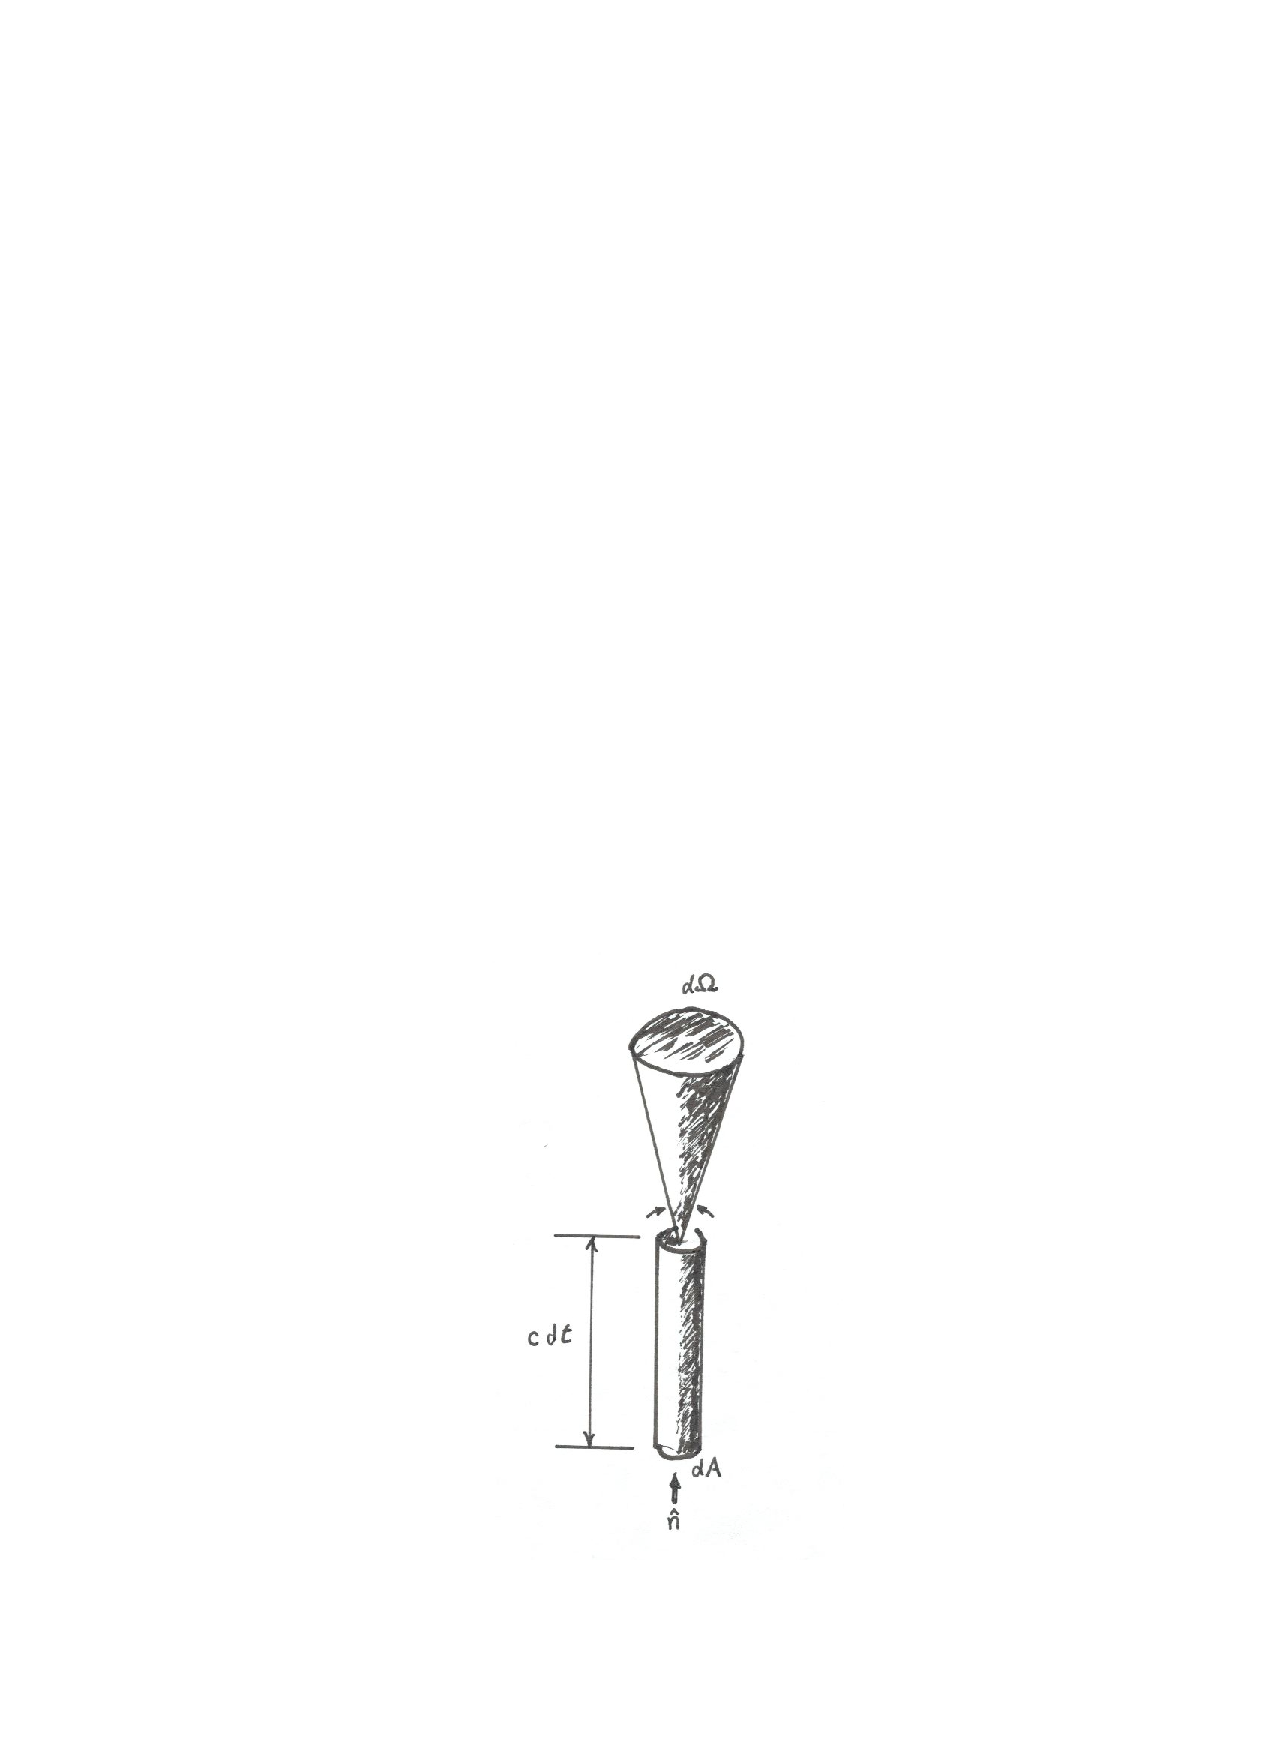
\includegraphics{intensity-schematic}
\caption{\label{f.intensity-schematic}Schematic of a pencil of radiation propagating into an angle $\dif\Omega$.}
\end{figure}

The energy density per frequency $u_{\nu}$ can be defined as $\dif E/(c \dif t\,\dif A\,\dif\nu)$; comparing this with the definition of $I_{\nu}$, we see that (for a blackbody)
\begin{equation}\label{e.radiation-energy-density}
u_{\nu} = \frac{1}{c}\int I_{\nu}\,\dif\Omega = \frac{8\pi h\nu^{3}}{c^{3}}\left[\exp\left(\frac{h\nu}{\kB T}\right)-1\right]^{-1}.
\end{equation}
The total energy density can be found by integrating over all frequencies, giving
\[ u = \left[\frac{8\pi^{5}\kB^{4}}{15 h^{3}c^{3}}\right] T^{4}\equiv aT^{4} \]
in agreement with statistical mechanics.

The next quantity to define is the \emph{flux} of energy, with direction $\unitk$, per unit time $\dif t$,  per unit area $\dif A$, and per frequency interval $\dif\nu$,
\begin{equation}\label{e.radiation-flux}
\bvec{F}_{\nu} = \int \unitk I_{\nu} \,\dif\Omega.
\end{equation}
Note that $\bvec{F}_{\nu}$ is a vector;  the net flux along a direction \unitn\ is
\[ F_{\nu} = \int I_{\nu}(\unitn\cdot\unitk)\dif\Omega. \]
If we take our polar angle with respect to $\unitk$, then $(\unitn\cdot\unitk)\,\dif\Omega = \cos\theta\,\sin\theta\,\dif\theta\,\dif \phi$; defining the direction cosine $\mu = \cos\theta$, this becomes 
\[ (\unitn\cdot\unitk)\,\dif\Omega = 2\pi \mu\,\dif\mu. \]
Note that if the radiation field is isotropic then $F_{\nu}=0$: there must be some anisotropy in the radiation field to generate a net flux.

For blackbody radiation, if we only integrate over outgoing directions, $0\le \mu\le 1$, as would be the case for thermal radiation emerging from a \emph{hohlraum},
\[ F_{\nu} = \pi B_{\nu}.\]
Integrating this $F_{\nu}$ over all frequencies, we recover the Stefan-Boltzmann formula,
\[ F = \left(\frac{ac}{4}\right) T^{4} \equiv \sigma_{\mathrm{SB}} T^{4}, \]
where $\sigma_{\mathrm{SB}}$ is the Stefan-Boltzmann constant.

Finally, let's look at the momentum flux transported along direction \unitk, per unit time $\dif t$, per unit area $\dif A$, and per unit frequency interval $\dif\nu$.  Since for a photon, $E = pc$, we divide the energy flux by $c$.
This is a \emph{tensor},
\begin{equation}\label{e.radiation-pressure-tensor}
\btens{P}_{\nu} = \frac{1}{c}\int \unitk\unitk I_{\nu}\dif\Omega.
\end{equation}
The net momentum flux along a direction \unitn\ is then
\[ P_{\nu} = \frac{1}{c}\int (\unitn\cdot\unitk)(\unitn\cdot\unitk) I_{\nu}\,\dif \Omega = \frac{2\pi}{c}\int_{-1}^{1} I_{\nu}\mu^{2}\,\dif\mu. \]
For blackbody radiation, 
\[ P_{\nu} = \frac{4\pi}{3c} B_{\nu}  = \frac{1}{3}u_{\nu}\]
and we may integrate this over frequency to obtain $P = u/3$, the standard result from thermodynamics.

\section{Some simple estimates}

We argued in the previous section that the solar interior is quite opaque. Naively, we might imagine some radiative transition, e.g. bremsstrahlung, emitting a photon.  The photon speeds away at $c$, but it doesn't get very far before being absorbed or scattered by another particle. A new photon, either due to emission or scattering, will be emitted at some random direction, and the whole process repeats. This is just a description of a \emph{random walk}. 

For some simple estimate, let's assume that the hop is the same for all photons, regardless of frequency or ambient temperature. If the hop length is $\ell$, then we know that the total path length to get from the center to the surface is $\Rsun(\Rsun/\ell)$ and the time for this to occur is $\Rsun^{2}/\ell/c$. What is a good estimate for $\ell$?  Consider a planar electromagnetic wave incident on a collection of scatterers. If these scatterers are uncorrelated, then the probability of scattering is just the number of scatterers times the probability for scattering from a single scatterer.  Define the probability of scattering as
\begin{equation}\label{e.scattering-probability}
\mathcal{P} = N\times\left(\frac{\textrm{energy scattered per unit time by one scatterer}}{\textrm{energy incident per unit time per unit area}}\right)\frac{1}{ \mathcal{A}}
\end{equation}
where $\mathcal{A}$ is the area normal to the propagation direction \unitk\ of the volume containing the $N$ scatterers.  The quantity in parenthesis is just the definition of the cross-section $\sigma$. Furthermore, if we set $\mathcal{P} = 1$, then the total number of scatters is just $N = n\times \mathcal{A}\times \ell$, where $n$ is the number density of scatterers. Thus we define the \emph{mean free path},
\begin{equation}\label{e.mean-free-path}
\ell = \frac{1}{n\sigma}.
\end{equation}
In stellar work, it is more convenient to use mass density rather than number density.  Writing $n = Y\rho/\mb$, where $Y$ is the abundance of scatterers, we have
\[ \ell = \rho^{-1} \left(\frac{\sigma}{\mu\mb}\right) \equiv (\rho\kappa) \]
where $\kappa$ is the \emph{opacity} and has dimensions $[\kappa]\sim[\cm^{2}\nsp\gram^{-1}]$.

The opacity in the stellar interior is set by a large number of processes; Thomson scattering, free-free absorption, atomic absorption and photoionization.  In general, the cross-section depends on the ambient temperature and density and the frequency of the photon. For crude estimates, we can use Thomson scattering, which is scattering from non-relativistic electrons when the photon energy is sufficiently low that we can neglect the recoil of the electron.  The cross-section for Thomson scattering is 
\begin{equation}\label{e.Thomson-cross-section}
\sigma_{\mathrm{Th}} = \frac{8\pi}{3}\left(\frac{e^{2}}{m_{e}c^{2}}\right)^{2} = 0.665 \times 10^{-24} \nsp\cm^{2}.
\end{equation}
The opacity for Thomson scattering is then
\[ \kappa_{\mathrm{Th}} = (0.4\nsp\cm^{2}\nsp\gram^{-1}) Y_{e}. \]
The factor of $Y_{e}$ is because the scattering is from electrons, which are much lighter than nuclei and therefore easier for an incident wave to shake.

Further processes will only make $\ell$ shorter than our estimate using Thomson scattering.  Now, over the length of a hop $\ell$ there will only be the most minute of variations with respect to temperature and density.  As a result, the conditions are nearly isotropic, so we indeed expect the radiation to come into thermal equilibrium with the ambient material.  But not perfectly---otherwise there would be zero net heat flux!  It is the small anisotropy that gives rise to the transport of energy.  Let's imagine a small cube of material, with the size of this cube being $\ell$.  Because we are so very nearly isotropic and in thermal equilibrium, the flux through any one face of this cube must be $(c/6)u$.  Now suppose we have an adjacent cube. It is emitting into our cube a flux $(c/6) u(x')$.  Hence, the net flux across the face (taken to be at $x=0$) between these two cells is
\begin{eqnarray}
	F &\approx& \frac{c}{6} u(x-\ell) - \frac{c}{6} u (x+\ell)\nonumber \\
	&=& -\frac{1}{3}c\ell\frac{\dif u}{\dif x}.\label{e.rad-diffusion-simple}
\end{eqnarray}
This is a diffusion equation with coefficient $c/(3\rho\kappa)$.  Of course, this is very crude, as it neglects the variation in cross section with the properties of the ambient medium and with the photon frequency.  Nonetheless, this is basically what happens when convection is absent; heat diffuses with a coefficient given by some suitably defined average over all sources of opacity. 

\section{Equation of Transfer}

We're now ready to formalize the crude work in the previous section.
In the absence of interactions with matter, the specific intensity $I_{\nu}$ is conserved along a ray propagating in direction \unitk: $\dif I_{\nu}/\dif s = c^{-1}\partial_{t}I_{\nu} + \unitk\cdot\grad I_{\nu} = 0$. If matter is present, it can do three things to change $I_{\nu}$.
\begin{description}
\item[emit] Matter may spontaneously emit photons and add to the beam: $\dif I_{\nu}\dif s = \rho\varepsilon_{\nu}/(4\pi)$. Here $\varepsilon_{\nu}$ is the energy spontaneously emitted per unit frequency per unit time per unit mass: this term represents the energy added to the beam along a path $\dif s$.  The factor of $4\pi$ is to make this term per steradian.

\item[absorb] Photons have a chance of being absorbed or scattered out of the beam: $\dif I_{\nu}/\dif s = -\rho\kappa_{\nu}I_{\nu}$. Here the right-hand side is the energy removed from the beam along a path $\dif s$ with $\kappa_{\nu} = \kappa_{\nu}^{\mathrm{abs}} + \kappa_{\nu}^{\mathrm{sca}}$ being the total opacity (absorption plus scattering). The dimensions of opacity are clearly $[\kappa_{\nu}] \sim [\cm^{2}/\gram]$. (If we had stimulated emission, this would be a \emph{negative} $\kappa_{\nu}$.)

\item[scatter] Photons may be scattered into the beam from other directions: $\dif I_{\nu}/\dif s = \rho\kappa_{\nu}^{\mathrm{sca}}\phi_{\nu}$. If the scattering is isotropic, then
\begin{equation}\label{e.isosca}
\phi_{\nu} = \frac{1}{4\pi}\int_{0}^{2\pi}\!\!\!\int_{0}^{\pi} I_{\nu}\,\dif\phi\,\sin\theta\,\dif\theta \equiv J_{\nu},
\end{equation}
where $J_{\nu}$ is the mean intensity: the scattering redistributes the energy over all angles.
\end{description}
Putting all these terms together gives us the \emph{equation of transfer},
\begin{equation}\label{e.transfer}
\frac{1}{c}\partial_{t}I_{\nu} + \unitk\cdot\grad I_{\nu} = \rho \frac{\varepsilon_{\nu}}{4\pi} - \rho\kappa_{\nu} I_{\nu} + \rho\kappa_{\nu}^{\mathrm{sca}}\phi_{\nu}
\end{equation}
for the specific intensity $I_{\nu}$.

\subsection{Radiative equilibrium} 
The emissivity $\varepsilon_{\nu}$ and the opacity $\kappa_{\nu}$ describe how the radiation interacts with matter. A condition of steady-state is that the gas not gain or lose energy to the radiation. This requires balancing
\[ \left(\textrm{energy emitted per unit volume}\right) = \rho\int\frac{\varepsilon_{\nu}}{4\pi}\,\dif\nu\,\dif\Omega\] 
with
\[ \left(\textrm{energy absorbed per unit volume}\right) = \rho\int \kappa_{\nu}^{\mathrm{abs}} I_{\nu}\,\dif\nu\,\dif\Omega,\]
or
\begin{equation}\label{e.rad-equil}
\int_{0}^{\infty}\! \left(\frac{\varepsilon_{\nu}}{4\pi} - \kappa_{\nu}^{\mathrm{abs}} J_{\nu}\right)\,\dif\nu = 0.
\end{equation}
Here we assume $\varepsilon_{\nu}$ does not depend on angle. We don't include scattering because it doesn't transfer energy between the radiation and the gas.

Now suppose that the level populations of the matter are in thermal equilibrium and can be described by a temperature $T$.  In that case, detailed balance must hold, so that
\begin{equation}\label{e.detail-balance}
\frac{\varepsilon_{\nu}}{4\pi\kappa_{\nu}^{\mathrm{abs}}} = B_{\nu}(T),
\end{equation}
where $B_{\nu}(T)$ is the Planck function. This defines \emph{local thermodynamic equilibrium (LTE)}. If the radiation field is, in addition, described by a Planck function \emph{at the same temperature} then we would have complete thermodynamic equilibrium.

\subsection{Optical depth}

Consider a ray directed into a medium in steady-state ($\partial_{t}\to 0$).  In the absence of emission ($\varepsilon_{\nu}=0$) or scattering ($\kappa_{\nu}^{\mathrm{sca}}=0$) equation~(\ref{e.transfer}) takes a particularly simple form:
\begin{equation}\label{e.transfer-optical-depth}
\frac{\dif I_{\nu}}{\dif \tau_{\nu}} = -I_{\nu}.
\end{equation}
Here we have set $\unitk\cdot\grad = (\dif/\dif s)$, where $\dif s$ is a infinetesimal along the path of the ray, and further have defined the \emph{optical depth} as
\begin{equation}\label{e.optical-depth-def}
\tau_{\nu} = \int \rho\kappa_{\nu}\,\dif s.
\end{equation}
Note that $\tau_{\nu}$ is dimensionless. Taking $\rho$ and $\kappa_{\nu}$ as given, equation~(\ref{e.transfer-optical-depth}) has a simple solution,
\[ I_{\nu}(\tau_{\nu}) = I_{\nu}(0)\exp\left(-\tau_{\nu}\right). \]
Note that $\rho\kappa=\ell^{-1}$, so equation~(\ref{e.optical-depth-def}) is just $\tau = \int \dif s/\ell$, i.e., it expresses distance by counting the number of mean free pathlengths traversed.

\subsection{Source function}

Having defined the optical depth, we can now add the emissivity $\varepsilon_{\nu}$ and scattering term (henceforth we will assume isotropic scattering) to equation~(\ref{e.transfer-optical-depth}) to obtain
\begin{equation}\label{e.transfer-with-source}
\frac{\dif I_{\nu}}{\dif \tau_{\nu}} = S_{\nu}-I_{\nu},
\end{equation}
where 
\begin{equation}\label{e.source-fcn-def}
S_{\nu} \equiv \frac{1}{\kappa_{\nu}}\left(\frac{\varepsilon_{\nu}}{4\pi} + \kappa_{\nu}^{\mathrm{sca}}J_{\nu}\right)
\end{equation}
is the \emph{source function}. 
We can formally solve equation~(\ref{e.transfer-with-source}), obtaining
\[ I_{\nu} = I_{\nu}(0)\exp(-\tau_{\nu}) + \int_{0}^{\tau_{\nu}} S_{\nu} \exp(-t)\,\dif t. \]
In reality, there is typically some complicated mapping between position and $\tau$, so the transfer equation cannot be solved so simply.

\section[Diffusion Approximation]{Diffusion Approximation and the Rosseland Mean Opacity}

At large optical depth, such as deep in a stellar interior, the radiation field is in thermal equilibrium, so that $I_{\nu} = S_{\nu} = B_{\nu}$. To see this, consider the relative scales of terms in the transfer equation.
\begin{center}\begin{tabular}{ccccccccc}
$\displaystyle \frac{1}{c}\frac{\partial I_{\nu}}{\partial t}$ & + &
$\displaystyle  \unitk\cdot\grad I_{\nu}$ & = &
$\displaystyle\rho\frac{\varepsilon_{\nu}}{4\pi} $ & $-$ & 
$\displaystyle \rho\kappa_{\nu} I_{\nu}$ & $+$ &
$\displaystyle \rho\kappa_{\nu}^{\mathrm{sca}} J_{\nu}$\\
I & & II & & III & & IV & & V
\end{tabular}
\end{center}
On the left-hand side, term I scales as $I_{\nu}/(c t_{\odot})$, where $t_{\odot}$ is the evolutionary timescale of the sun (\Giga\yr), and term II scales as $I_{\nu}/R_{\odot}$. On the right-hand side, term IV scales at $I_{\nu}/\ell$.  Hence the ratio of terms of term II to term IV is $\ell/R_{\odot}\ll 1$ and that of term I to term IV is $\ell/\Giga\parsec\ll 1$. In addition, stellar properties change negligibly on scales of a mean-free path, so conditions are nearly isotopic over much of the interior and $I_{\nu} = J_{\nu}$. Hence $I_{\nu} = J_{\nu} = S_{\nu}$, and inserting the relation between $\varepsilon_{\nu}$ and $\kappa_{\nu}^{\mathrm{abs}}$ from detailed balance, eq.~(\ref{e.detail-balance}), into equation~(\ref{e.source-fcn-def}) implies that $S_{\nu} = B_{\nu}$.

If the radiation field is perfectly isotropic there is no flux, however, so we must have some small anisotropy. Let's write $I_{\nu}$ as a thermal term plus a correction, 
\[ I_{\nu} = B_{\nu}(T) + I^{(1)}. \]
Substituting this into the steady-state equation of transfer,
\[ \frac{1}{\rho\kappa_{\nu}}\unitk\cdot\grad I_{\nu}  = S_{\nu} - I_{\nu}\]
and canceling the $B_{\nu}$ on the right-hand side, we obtain
\begin{equation}\label{e.rad-diffusion-1}
I_{\nu}^{(1)} = -\frac{1}{\rho\kappa_{\nu}} \unitk\cdot\grad B_{\nu} = -\frac{1}{\rho\kappa_{\nu}} \frac{\partial B_{\nu}}{\partial T} \unitk\cdot\grad T.
\end{equation}
This is anisotropic: the energy transport is largest in the direction ``down'' the temperature gradient. Let's get the net flux: multiplying equation~(\ref{e.rad-diffusion-1}) by $\unitn\cdot\unitk$, replacing the two dot products by the angle cosine $\mu$, and integrating over $\dif \Omega = 2\pi \dif\mu$, we obtain
\begin{equation}\label{e.rad-diffusion-2}
\bvec{F}_{\nu} = -\frac{4\pi}{3}\frac{1}{\rho}\left[\frac{1}{\kappa_{\nu}}\frac{\partial B_{\nu}}{\partial T}\right]\grad T.
\end{equation}
The quantity in $[\,]$ deserves a closer look. First, suppose $\kappa_{\nu}$ is independent of frequency. Then equation~(\ref{e.rad-diffusion-2}) means that the energy transport is greatest at the frequency where $\partial B_{\nu}/\partial T$ is maximum, and \emph{not} at the peak of the Planck spectrum. 

Let us define the \emph{Rosseland mean opacity} as
\[ \kappa_{\mathrm{R}} \equiv \left[\frac{\int\,\dif\nu\,\kappa_{\nu}^{-1}(\partial B_{\nu}/\partial T)}{\int \,\dif\nu\, (\partial B_{\nu}/\partial T)}\right]^{-1}. \]
We can use this to integrate equation~(\ref{e.rad-diffusion-2}) to obtain the total radiative flux,
\begin{equation}\label{e.rad-flux}
\bvec{F} = - \frac{4\pi}{3} \frac{1}{\rho\kappa_{\mathrm{R}}} \grad\left[\int\,\dif\nu\,B_{\nu}\right] = - \frac{1}{3} \frac{c}{\rho\kappa_{\mathrm{R}}} \grad aT^{4}.
\end{equation}
This is just our formula for radiation diffusion (eq.~[\ref{e.rad-diffusion-simple}]) that we obtained from physical arguments, but now we have an expression for the effective opacity $\kappa_{\mathrm{R}}$.

\section{Sources of Opacity}\label{s.opacity-sources}

The textbook enumerates many of the opacity sources. We already mentioned Thomson scattering. Another important one is free-free absorption, or inverse \emph{bremsstrahlung}. As an example of how these are computed, let's start with free-free emission. Consider the collision of an electron with an ion of charge $Ze$ with impact parameter $b$ (see Figure~\ref{f.scattering}).  In an impulse approximation, the electron receives an acceleration (perpendicular to its original direction of motion)
\[ \bvec{\dot{v}} = \frac{Ze^{2}}{me b^{2}}. \]
This acceleration leads to an emission of radiation; according to Larmor's formula, the power emitted is
\begin{equation}\label{e.larmor}
P(b) = \frac{2}{3}\frac{e^{2}}{c^{3}} |\bvec{\dot{v}}|^{2} = \frac{2}{3}\frac{Z^{2}e^{6}}{m_{e}^{2}c^{3}b^{4}}.
\end{equation}
The duration of the impulse is $\approx b/v$, so the total energy emitted is $E(b)\approx P(b)b/v$.  An electron moving at velocity $v$ will undergo $\approx 2\pi b\,\dif b \times v n_{I}$ collisions with impact parameters in a range $(b, b+\dif b)$ per unit time.  The total emissivity, \emph{for this impact parameter}, is
\begin{equation}\label{e.free-free-b}
	\rho \varepsilon_{b}\,\dif b \approx \left\{\int \; \frac{4\pi}{3} \frac{Z^{2}e^{6}n_{I}}{m_{e}^{2}c^{3}b^{2}}\,f(v)\,\dif^{3}v\right\}\dif b.
\end{equation}
Here $f(v)$ is the distribution function for electrons.  

Before going further, I want to clean up the physical constants.  First, recognize that $(8\pi/3) (e^{2}/m_{e}c^{2})^{2} = \sigma_{\mathrm{Th}}$, the Thomson cross section; I can also introduce factors of $\hbar$ to convert the other factor of $e^{2}$ into the fine-structure constant $\alpha$, giving
\begin{equation}\label{e.free-free-clean}
	\rho \varepsilon_{b}\,\dif b \approx \left\{\int \; \frac{1}{2b^{2}} Z^{2}\alpha \sigma_{\mathrm{Th}} \hbar c^{2} n_{I}\,f(v)\,\dif^{3}v\right\}\dif b.
\end{equation}
The emission of a single scattering with impact parameter $b$ has a strong frequency dependence, with most of the emission emitted at frequencies $\nu \approx 1/\delta t \approx v/b$. It is therefore convenient to convert equation~(\ref{e.free-free-b}) to a distribution over  $\nu$. To do this, we write $\dif b = |\dif b/\dif \nu|\dif \nu \approx (b^{2}/v) \dif\nu$. Inserting this into equation~(\ref{e.free-free-b}), and expanding 
\[
	f(v)\,\dif^{3}v = 4\pi n_{e}\left(\frac{m_{e}}{2\pi\kB T}\right)^{3/2}\exp\left(-\frac{m_{e}v^{2}}{2\kB T}\right) v^{2}\,\dif v
\]
then gives
\begin{equation}\label{e.free-free-w-int}
\rho \varepsilon_{\nu}\,\dif\nu \approx \left\{ n_{I}n_{e}\frac{Z^{2}\hbar c^{2}  \alpha \sigma_{\mathrm{Th}}}{\sqrt{2\pi}} \left(\frac{m_{e}}{\kB T}\right)^{3/2} \int_{v_{0}}^{\infty} \;\exp\left(-\frac{m_{e}v^{2}}{2\kB T}\right)\,v\,\dif v\right\}\,\dif \nu.
\end{equation}
Why is there a lower limit on the integral? In order to emit a photon at all, we need $m_{e}v^{2}/2 > \hbar \nu$.  Performing the integral gives the frequency-specific emissivity (I'll drop the factor of $\sqrt{2\pi}$, since this is only a rough approximation),
\begin{equation}\label{e.free-free-w}
\rho \varepsilon_{\nu} \approx n_{I}n_{e} Z^{2}\hbar c^{2}  \alpha \sigma_{\mathrm{Th}} \left(\frac{m_{e}}{\kB T}\right)^{1/2}\,\exp\left(-\frac{\hbar\nu}{\kB T}\right).
\end{equation}
Given the emissivity, we can now obtain the absorption via detailed balance (eq.~[\ref{e.detail-balance}]),
\[ \kappa_{\nu}^{\mathrm{ff}} = \frac{\varepsilon_{\nu}}{4\pi B_{\nu}(T)} . \]

\section{Exercises}
\begin{enumerate}
\item If we regard the sun as a large cavity filled with photons, estimate the total energy stored in the radiation field.  If the sun were suddenly to become completely transparent, what would be the resulting luminosity?

\item Explain on physical grounds why the flux for a grey opacity would be greatest at the frequency for which $\partial B_{\nu}/\partial T$, rather than $B_{\nu}$, is maximized.

\item Suppose both free-free absorption ($\kappa^{\mathrm{ff}}_{\nu}$) and Thomson scattering ($\kappa^{\mathrm{Th}}_{\nu}$) contribute to the opacity. Denote by $\langle\,\rangle$ the Rosseland averaging of an opacity.  Does $\langle \kappa^{\mathrm{ff}}_{\nu} + \kappa^{\mathrm{Th}}_{\nu}\rangle = \langle\kappa^{\mathrm{ff}}_{\nu}\rangle+\langle\kappa^{\mathrm{Th}}_{\nu}\rangle$? 

Now suppose that $\kappa^{\mathrm{ff}}_{\nu}$ is due to free-free absorption on two different ion species (denoted below by subscripts ``1'' and ``2'') with different charge number $Z$.  In this case does $\langle \kappa^{\mathrm{ff}}_{\nu,1} + \kappa^{\mathrm{ff}}_{\nu,2}\rangle = \langle\kappa^{\mathrm{ff}}_{\nu,1}\rangle+\langle\kappa^{\mathrm{ff}}_{\nu,2}\rangle$?

\item Estimate the ratio of the conduction heat flux carried by electrons to that carried by photons, at conditions appropriate to the solar center.  In the low-density (non-degenerate) limit the conductivity is roughly \citep{spitzer62:_physic}
\[
K \approx 3.1\ee{12}  \left(\frac{T}{10^{7}\nsp\K}\right)^{5/2}\frac{1}{Z}\nsp\ergs\usp\K^{-1}\nsp\cm^{-1}\nsp\second^{-1}.
\]
Now suppose we wish to write a single equation for heat transport,
\[
\bvec{F} =  -\frac{4}{3} \frac{acT^{3}}{\rho\kappa_{\mathrm{total}}}\grad T.
 \]
Derive an expression for $\kappa_{\mathrm{total}}$ in terms of the electron conductivity $K$ and the free-free opacity $\kappa_{\mathrm{ff}}$.  

\end{enumerate}
